\documentclass[12pt]{article}

%Packages
\usepackage{graphicx} %For graph insertion
\usepackage[margin=1in]{geometry} %Set margins
\usepackage[section]{placeins} %Place objects in section
\usepackage{authblk} %Extend intro
\usepackage{amsmath}
\usepackage[bottom]{footmisc} %Bottom footnote
\usepackage{subfig} %side by side
\usepackage{apacite} %APA style
\usepackage{natbib} %cite special
\usepackage[T1]{fontenc} %Croatian citation
\usepackage{currvita} %Croatian
\usepackage{titlesec} %Get subsubsection
\usepackage{setspace}%Set spacing
\usepackage{rotating} %Landscape table
\renewcommand{\floatpagefraction}{.8}%
%Title
\title{Home Sharing in New York City: Impact on Hotel, Rental, and Welfare}
\author{Tai Nguyen\\
Advisor Giri Parameswaran} %Author
\date{May 2, 2019} %Date
\affil{Department of Economics, Haverford College}

%Double spacing for body 
\linespread{1.6}

%Document begins
\begin{document} 
	\begin{singlespace} %Begin single space
	\clearpage\maketitle %Make title
	\thispagestyle{empty} %No page number
	
	\begin{doublespace}
	\begin{abstract} %Abstract
		A major sector under the sharing economy, home sharing is a newly emerged concept. This paper explores how the growth of home sharing influences the temporary accommodation markets in New York City. Using monthly data spanning between 2015-2018 for Airbnb, I quantify the platform short- and long-term impact on hotel and rental housing. Overall, though little substitution effect is discovered between home sharing and hotel, there is evidence of strong competitive pressure. OLS regression results find a 10\% increase in Airbnb supply to be associated with a 1.3\% decrease in hotel price and a 1.2\% decrease in hotel revenue, making the incumbent industry cheaper and less profitable. From a deadweight loss savings perspective, daily welfare benefit created by home sharing is measured around \$8,000 during the period, which is not economically significant. Controlling for neighborhood and month, an increase in Airbnb supply is also found to raise median asking price across all types of rental units considered, making rental less affordable. Additionally, a hedonic regression of Airbnb listings uncovers the main price determinants of New York accommodation, including number of reviews and centrality. My paper adds to previous literature by focusing on the impact of home sharing in a large, yet understudied urban area.
		 
		\noindent\textbf{Keywords:} Airbnb, sharing economy, New York, home sharing, hotel, rental, welfare\\
	\end{abstract}
	\clearpage
	
	\begin{frame}{}
		\section*{\centering Acknowledgements}
			\indent
			This research is not possible without data provided by Inside Airbnb, Smith Travel Research, Zillow, and other organizations that generously made their data available for my study.\\
			
			\par \noindent
			Thank you to Haverford College, especially the Economics Department, for teaching me to be curious and to think critically.\\
			
			\par \noindent
			I would like to thank professor Giri Parameswaran for your knowledge, wisdom, and encouragement in writing this paper. Working with you has been an incredible learning opportunity. Thank you professor David Owens for your helpful feedback at the beginning stages of this project.\\
			
			\par \noindent
			And to professor Weiwen Miao and professor Eric Gaus, for giving me the tools to answer questions and instill in me a love for data and Statistics.\\
			
			\par \noindent
			Lastly, to my wonderful parents, for their sacrifices to give me the opportunities they never had. To my brother Victor, Grace, and others who have made this journey so memorable, thank you.
			
	
	\end{frame}
	\end{doublespace}
	\clearpage
	
	\tableofcontents %Table of Contents
	\clearpage
	
	\end{singlespace} %End single space
	
	\section{Introduction}  %Introduction
		The concept of home sharing, offering an entire house or a portion of it online in exchange for compensation, is a newly emerged concept. Facilitated by technology, sharing economy platforms enabled transactions between strangers. In the past decade, platforms such as Uber, Lyft, and Airbnb have become a major part of modern life, shaping consumers and markets\footnote{Notable examples include the impact of ride sharing on traffic congestion \citep{li2016ride}, Uber on taxicabs in Taiwan \citep{chang2017economic}, and Craigslist on waste reduction in California and Texas \citep{fremstad2017does}.}. In the case of home sharing, economists have found it to have an impact on both incumbent firms \citep{zervas2017rise, farronato2018welfare} and the housing market \citep{horn2017home, barron2018sharing}. Using evidence from web-scraped Airbnb data, this paper is an examination of home sharing impact in New York City, a highly populated urban area. This adds to the growing body of literature on the multitude ways in which home sharing might affect short- and long-term accommodations\footnote{By our definition, hotel and home sharing, accommodation offered for as little as one day, are under the short-term structure. The rental housing market, offered for at least 30 days, are under the long-term categorization.}. By employing different regression techniques and a competition model, I test conclusions found in previous works about the impact of home sharing and extend the data to quantify its welfare effects from a deadweight loss perspective.
		
		\par
		In New York City, as in other major U.S. urban areas, regulations around housing remain a contentious debate \citep{weiser2019judge, said2018leaner}. Supporters of home sharing speak to the benefits of earning extra income and having (often) cheaper alternatives to hotels\footnote{From our data, the average hotel was 1.7 times more expensive than the average Airbnb.}. Meanwhile, its critics argue that platforms like Airbnb directly raise rent prices and limit the number of rental units available, accentuating urban housing problems. As the government grapples with the decision to support or restrict these platforms, empirical knowledge on the recently emerged market phenomenon is important for implementing well-informed policy decisions.
		
		\par
		Besides housing shortage, taxation poses another problem for concern. Currently, though income reporting made on sharing economy platforms is mandated by the Internal Revenue Services (IRS), there is still great inconsistency across individuals and cities regarding income reporting \citep{cestnick2018navigating}. As government revenue crucially rely on taxes from traditional, well-regulated industries such as hotel and taxicab, a demand shift away from these incumbents bring up challenges in cities where sharing economy presence is the strongest \citep{zervas2017rise}. Urban housing, taxation, and welfare stand out as the main motivating factors behind my study.
		
		\par
		I investigate the short-term impact of Airbnb on both local hotel and rental housing between January 2015 and December 2018. Data was drawn from many sources, including Inside Airbnb, STR Global, StreetEasy, Zillow Research, and others. Descriptive statistics of Airbnb show potential evidence of hotel competition and illegal home sharing activities\footnote{Under New York state law, it is illegal for an apartment to be rented out for less than 30 days unless the permanent tenant is residing in the apartment at the same time \citep{weiser2019judge}} in New York City. The latter is the cause of multiple protests in June 2018 \citep{greenberg2018new}. For incumbent hotels, Airbnb's affordability (1.7 times cheaper) and continuing strong growth (Figures \ref{fig:AirbnbvsHotelGrowth} and \ref{fig:AirbnbSpread}) impose strong threats of substitution. For rental, data analysis finds results similar to what \citet{horn2017home} found in Boston. In particular, on December 6, 2019 in New York City, 86\% of hosts had a single simultaneous listing on Airbnb, suggesting that the majority of homeowners are participants seeking extra income by renting out their place. However, 14\% of hosts who own multiple listings had over one-third of all available rooms on the platform, suggesting that many also rent out their place commercially. These are units that would, otherwise, serve as available living space for local residents \citep{horn2017home}.
		
		\par
		As home sharing affects hotel and rental differently, I provide a theory to illustrate that effect. For hotels in New York City, high occupancy rates year-round signal low effect of substitution, though OLS regression results indicate that Airbnb does  assert competitive pressure on lodging: a 10\% increase in Airbnb supply is associated with a 1.3\% decrease in hotel average daily rate and a 1.2\% decrease in hotel revenue. In the long run, I find that Airbnb, on average, saves \$8,000 of daily deadweight loss during 2015-2018. Due to characteristics of my data, these results should be carefully considered. For rental, an increase in Airbnb supplied is found to raise rents across all housing types, an agreement with \citet{horn2017home} and \cite{barron2018sharing}. Other insights are found, including important price determinants of New York City accommodation. Overall, my contributions to growing literature on sharing economy are three-fold: (1) examining home sharing impact in an understudied market, (2) confirming results found in previous literature, and (3) adding on to the pros and cons debate around the sharing economy.
		
		\par
		The next section, Section 2, discusses previous literature done on the sharing economy and gives a brief overview of Airbnb. Here, I describe in detail other studies connected to home sharing. Section 3 provides a theory that sets the stage for my empirical method. Section 4 discusses different data sources and give important descriptive statistics about the data. To follow, Section 5 explains the construction of the hedonic price index estimation and outlines the OLS regressions. Section 6 describes empirical results, while Section 7 includes a robustness check. To conclude, Section 8 reiterates important findings and discusses important policy implications for home sharing.
		
	\section{Previous Literature} %Previous Lit
		\subsection{Peer-to-peer Sharing Economy}
			Previous economists credit technological innovations for the growth of sharing economy platforms. \citet{einav2016peer} points to their ability to solve core market design problems: efficiently matching buyers and sellers, setting competitive prices, and providing transactions that are safe and reliable. These are characteristics shared by popular platforms like Uber, Airbnb, and Craigslist. Across transportation, accommodation, and shopping, they disrupt traditional industries to create larger, faster, and more geographically diverse marketplaces. In doing so, modern consumers gain access to a wider and more personalized range of products and services \citep{einav2016peer}. While imperfection such as discrimination still exists on these marketplaces \citep{kakar2018visible}, most academic works agree on the welfare benefits come from enabling people to make use of underutilized resources by sharing.
			
			\par
			In a paper exploring the impact of ride sharing on traffic congestion, \citet{li2016ride} find the entry of Uber to be associated with a decrease in Commuter Stress Index. This result was tested for two-way causation (whether traffic congestion actually helped Uber expand) and found to be statistically significant. In another paper, \citet{kroft2014does} study the impact of Craigslist on local unemployment rates through an OLS regression model. Although finding evidence that Craigslist influences unemployment, the authors conclude that the efficient supply-demand matching platform reduced the apartment vacancy rates by 10\% between 2003 and 2007. This is an example of technology-enabled efficient market design. In another study of Craigslist, \citet{fremstad2017does} found a link between the platform and waste reduction in both California and Florida. Using county-level public waste data from the two states and a difference-in-differences strategy, \citet{fremstad2017does} finds that, on average, daily per capita waste fell by 0.37 pounds in counties after a Craigslist entry. As the platform promotes the reuse of durable secondhand goods, \citet{fremstad2017does} asserts that Craigslist has diverted millions of tons from the solid waste stream, saving Californians and Floridians hundreds of millions of dollars in waste collection and waste disposal. Positive environmental externality is a type of welfare improvement that compels my study.
			
		\subsection{Overview of Airbnb}
			Airbnb, founded in 2008, describes itself as a trusted accommodation marketplace for people to list, find, and book unique accommodations around the world – from a website or smart phone \citep{farronato2018welfare}. A decade after its first appearance in San Francisco, U.S., the platform now provides access to over 5 million unique listings in more than 81,000 cities and 191 countries (Airbnb Press Room). Like other peer-to-peer platforms, the technology-based company enables a previously rare transaction: the short-term rental of an apartment or room to strangers \citep{farronato2018welfare}. Guests search for listings that fit their preferences of price, location, and duration. Hosts rent out extra rooms as they have availability. A key built-in mechanism on the platform is a reputation system that helps both hosts and guests build trust through rating and reviewing each other after every transaction. Ratings are out of five stars, while written reviews are visible publicly. The feature maximizes the likelihood of a successful transaction and brings a sense of transparency to the marketplace. As accommodation is complex, Airbnb can sometimes fail to completely reduce search frictions such as listing heterogeneity or transactional costs \citep{einav2016peer}. \citet{horton2014misdirected} found that, even after buyers have identified the listing of interest, many Airbnb transactions still falls through because the seller rejects the buyer as they become unavailable or have simultaneous accepted another inquiry. This makes it difficult to correctly estimate Airbnb supply and demand at equilibrium.
			
			\par
			Currently, New York City is Airbnb's biggest domestic market (over 50,000 listings in August 2018). Its dominance sparks curiosity, as \citet{yang2017customers} highlights the platform’s untraditional characteristics through a marketing perspective. Compared to traditional hotels or even bed \& breakfasts, Airbnb hosts are often non-industry specialists, lack professional training, and act as agents of their own interests \citep{yang2017customers}. Despite these characteristics, Airbnb's rapidly increasing market shares in New York City is formidable (Figure \ref{fig:AirbnbvsHotelGrowth}). Studying how and why this accommodation platform has impacted traditional industries allow for new understanding of market competition, consumer behaviors, and the sharing economy.
			
		\subsection{Linkage to Accommodation Markets}
			The demand of U.S lodging industry moves closely with U.S. GDP \citep{wheaton1999real}. Economic principles dictate that, as GDP increases, demand for more goods and services follows, giving rise to more supply. Over the past 5 years, U.S lodging has been growing at a robust rate at 4.4\%, with over \$190 billion in 2018 revenue driven by increase in travel spending, corporate profit, and consumer spending (IBISWorld Report). Though witnessing great growth, the industry is also highly competitive and susceptible to economic and technological change \citep{kalnins2006markets}. Many journal and news articles speak to the competition challenge posed by Airbnb, HomeAway, and VRBO. \citet{zervas2017rise} found evidence suggesting that consumers are increasingly substituting Airbnb stays for lower-end hotels in Texas, possibly due to the latter option “providing more utility for the same price." Based on this insight, authors argue that sharing economy platforms have the potential to transformatively increase social welfare. Between hosts who make incremental income by renting properties, guests who choose Airbnb as a cheaper alternative to hotel, and consumers who benefit from hotel quality improvement and affordability, home sharing platforms seem to benefit a large population of users around the world. My paper examines welfare from a deadweight loss perspective, assuming that home sharing perfectly absorbs burden created by a hotel price increase.
			
			\par
			The impact of home sharing on the hotel industry is not comparable to its impact on the local rental market. As \citet{horn2017home} observe, consumers do not consider short- (as few as 1 day) and long-term (as few as 30 days) accommodations to be similar goods. A visitor from Boston's decision to rent a room for a night or two in New York City does not affect her preference for permanent housing in either city \citep{horn2017home}. Meanwhile, host behaviors change with the rise of Airbnb, with more hosts expected to list their unit for short-term home sharing instead of renting out long-term to local residents. This phenomenon is discussed in more details in Section 3, with home sharing raising rents as a short-term effect observed by our empirical results. For municipal officials, regulating the housing market and their affordability are crucial to solving urban problems in highly-populated cities.
			
		\subsection{Previous Empirical Studies on Home Sharing}
			With the emergence of accommodation marketplaces being recent, few empirical studies have been conducted to realize their economic impact. One of the most prominent works in this sector was done by \citet{zervas2017rise}, who employs a difference-in-differences method to find the negative association between Airbnb supply and local hotel revenues in Texas. Fixed effects were taken at both a city and year-month level. Combining data from Airbnb website, the Texas Comptroller office, STR and the U.S Census Bureau, \citet{zervas2017rise} found a 10\% increase in Airbnb listings to be associated with a 0.39\% decrease in monthly hotel revenue. In Austin, the Texas city where Airbnb saw greatest growth, from 450 listings in 2010 to 8,500 listings in 2014, authors estimate a 10\% negative shock to Texas hotel revenue accumulated in the same period. These results are consistent with a substitution hypothesis between Airbnb and hotel, which was also found to differ among segments. By using interaction terms between hotel type and Airbnb supply, authors finds luxury hotels to be least affected by the platform, motivated by the insight that luxury hotels are least comparable to Airbnb based on average room price and amenities. In our analysis, a similar magnitude of substitution relationship between Airbnb and hotel is not found for New York City, though I suspect a few potential reasons for this effect.
			
			\par
			To quantify welfare, I follow similar estimation strategies put forth by \citet{farronato2018welfare}. As their stylized theoretical model points out, travelers benefit from Airbnb for two reasons: flexible sellers offering differentiated products, and hotel competition expanding the number of rooms available. Authors also find that entry of flexible supply is higher in cities like New York City, where demand fluctuates seasonally and hotel faces the biggest supply constraint.  Using daily data for 50 major U.S. cities, they estimate that Airbnb generates \$41 per room/night in consumer surplus, \$26 per room/night in host surplus, and reduce hotel profitability by 3.7\%. These numbers aggregate to a total welfare gain of \$137 million in 2014, a magnitude many times our results. From their method, a similar hedonic regression on nightly Airbnb price is employed in my paper. I complement \citet{farronato2018welfare} by including deadweight loss as another perspective to quantify welfare benefits of home sharing.
			
			\par
			On the rental market, \citet{horn2017home} is a study that investigates the short-term impact of home sharing growth on rentals in local neighborhoods of Boston. Using web-scraped Airbnb data and Rainmakers Insights, Inc., the authors employed a log-linear regression model to find that Airbnb density does affect rent price in the city. A one standard deviation increase in Airbnb density is found to be associated with a 0.4\% raise in asking-price. \citet{barron2018sharing} found a similarly positive association, which our OLS regression results confirm. For Boston, the authors discuss the inclusion of census tract fixed effects as a way to remove the effect of static rent differentials \citep{horn2017home}. Additionally, they mention an important source of omitted variable bias in change of neighborhood popularity, as prices of an Airbnb listing and rental apartment could see a positive shock by being in the same popular neighborhood. Regardless of the subject of study, each geographic area in the U.S. holds unique economic opportunities and legislations, all of which are important controls to consider. To ensure robust results as well as controlling for local differentials, I consider neighborhood fixed effects in my regression model.
			
			\par
			Compared to long-term rentals, \citet{coles2017airbnb} find centrality to be a predictor of Airbnb listing location in New York City and that short-term rentals do not appear as profitable as many assume. To capture centrality, authors compute a few metrics related to Airbnb listing intensity (percentage of listings in the radius) and proximity from central Manhattan (kilometers from the Empire State Building). Though it disperses gradually, usage was found to be heaviest in central neighborhoods of Manhattan and Northern Brooklyn, an agreement with Figure \ref{fig:AirbnbSpread} from the data. In 2016, booked listings were considerably more geographically dispersed than hotels, though hotels also appear to be more centralized due to zoning rules that contain them in commercially zoned neighborhoods \footnote{New York City geographically contain different commercial activities into 8 commercial districts based on their functional similarities and location requirements. For example, small retail and service shops appear in C1 and C12 districts while C4 is reserved for borough-wide regional retail centers. Source: https://www1.nyc.gov/site/planning/zoning/districts-tools/commercial-districts-c1-c8.page.} Two-thirds of hotels are located in Manhattan compared to 54\% of Airbnb booked listings. To capture profitability, \citet{coles2017airbnb} found the listing-weighted average ratio of median nightly rents to long-term daily rents to be 1.7 across neighborhoods. Airbnb is only about 1.7 times as profitable as hotel, so hosts would have to have their homes booked over 216 days a year to match long-term rental revenue \footnote{Excluded from this profit calculation are extra operational costs related to cleaning, depreciation from use, "broker fee" imposed by Airbnb, and other charges \citep{muller2014economic}}.
			
			\par
			In previous empirical studies, authors have used proprietary data or employed advanced computer techniques to extract the exact supply of Airbnb. Some researchers, similar to us, use Inside Airbnb \citep{coles2017airbnb, gurran2017tourists, kakar2018visible}, while others crawl the web themselves \citep{barron2018sharing, zervas2017rise}. Between these two sources, proprietary data is the only way to accurately know Airbnb demand, listings that were actually booked. Furthermore, it is also important to note that specific data related to hotel profitability (ie. hotel revenues and hotel pricing) will lack transparency. Though STR provides a good overview of the hotel industry, it does not cover all possible lodging in a city. These are all nuances related to data collection that have great implications for our methodology and results.
			
	\section{Theory} %Theory
		\subsection{Hotel Competition}
			In the model, hotel and home sharing are considered to be differentiated goods, products that fulfill the same need while not necessarily having identical features. The demand for both are determined by the seasonal trend and variability in number of traveling passengers. From the data, the average Airbnb unit is almost two times as cheap as the average hotel in New York City. As consumers in the market move down in price tier, home sharing and hotel become increasingly less differentiated. When consumers view these goods as substitutes, they rationally choose the one that provides them the same utility for a cheaper price. This is where the home sharing platform exerts the most pressure on hotel.
			
			\par
			In the short run, a hotel has options to deal with Airbnb growth, including a price response, an occupancy response, or a combination of both \citep{zervas2017rise}. Since hotel revenue per available room (RevPAR) is a product of occupancy rate and average daily price (ADR), a hotel that does not respond to a demand shock caused by home sharing would face a decrease in occupancy rate. Savvy hotel managers, however, could maintain occupancy by choosing to reduce room supply or to reduce price. The latter option results in a welfare gain for all consumers seeking accommodation, whether they use Airbnb or not. The lodging industry's high fixed cost and low marginal cost signal that hotel managers have few reasons to go with the first choice. For an available room, it is better to fill it - even at a low price - than to not fill it at all. Later in the paper, I test these short-term effects by regressing these hotel outcomes against Airbnb supply with a month fixed effects.

		\begin{figure}[!htbp] %Figure competition model
			\vspace{.2in}
			\begin{center}
				\caption{Hotel Competition Model} %caption* removes figure number
				\label{fig:HotelCompetition}
				\includegraphics[width=0.7\textwidth]{Slide1.jpeg}
				\begin{equation}
					Welfare = DWL = \frac{1}{2} \times  \bigtriangleup Q \times \bigtriangleup P
				\end{equation}
			\end{center}
			%\vspace{-.2in}
		\end{figure}
		
			\par
			In the long run, I consider a situation where home sharing does not exist. In Figure \ref{fig:HotelCompetition}, hotel equilibrium starts at $Q_0$ and $P_0$.  When hotel raises prices, the demand curve shifts down, creating a new equilibrium at $Q_1$ and $P_1$. Under this state, a deadweight loss incurs to all participants in the short-term accommodation market where everyone is worse off. As home sharing exists, I hypothesize that Airbnb fully absorbs this deadweight loss because it could flexibly scale supply to match demand. The empirical strategy to quantifying this deadweight loss is highlighted in Section 5.3.
						
		
		\subsection{Rental Term Structure}
		Home sharing and hotel target the short end of the rental term structure while rental housing targets the long end. Traditionally, these two modes of accommodations have been kept separate because there has not been a reliable market for short-term home sharing until the rise of Airbnb and VRBO. There existed complete market segmentation, where hosts could not freely move between the term structures \citep{horn2017home}. Within legal constraints\footnote{New York City zoning laws}, however, internet-enabled platforms have allowed for a rare fluidity in the market. My inquiry focuses on the fact that homeowners are utility maximizers.
		
		\par
		On a particular day, a peer host decides whether to make their home available for rent. She is responsive to market conditions, hosting short-term when demand for accommodation and prices are high, and making other choices when prices are low. Often, the daily rate gained from home sharing is expected to exceed the daily rate of longer-term accommodations. \citet{horn2017home} regards this as the "home sharing premium", which is reflected in our data. Between 2015 and 2018, the mean price of an Airbnb unit in Manhattan was \$150 per night, while the mean price of a Manhattan rental was \$3,296 per month, or approximately \$110 per night (Table \ref{tab:AirbnbStat}). This resulted in a sharing premium of \$40 per night during the period\footnote{In order to match revenue of renting long-term, the average Airbnb host in New York City would need their rooms booked for at least 267 days in a calendar year.}.
		
		\par
		Utility maximization theory dictates that, if profits earned home sharing premium surpasses profits earned from long-term rental, homeowners will choose to participate in the home sharing market. In other words, as hosts desire to gain the home sharing premium, it is reasonable expect the supply for rental housing to be affected. I hypothesize that the growth of home sharing in New York City will result fewer units available for rent, shifting the supply curve upwards. In the competition model in Figure \ref{fig:RentalSupply}, increase in price is expected to follow an upward shift in rental supply. In other words, rents will increase as a result of there being fewer rental housing units.
		
		\begin{figure}[!htbp] %Figure competition model
			\begin{center}
				\caption{Rental Supply} %caption* removes figure number
				\label{fig:RentalSupply}
				\includegraphics[width=0.68\textwidth]{Slide2.jpeg}
			\end{center}
			%\vspace{-.2in}
			\emph{The graph illustrates an upward shift in rental housing supply curve.}
		\end{figure}
		
		\par
		In \citet{coles2017airbnb} and \citet{horn2017home}, authors point out that the home sharing premium should decline as long-term accommodation prices rise. This is often a result of increasing demand or decreasing supply for accommodations at the long end of the term structure. Estimating the impact of home sharing on median asking rent and rental inventory requires the violation of a common assumption in housing economics: that the housing market is traditionally static and insensitive to short-term effects \citep{blank1953structure}. However, the emergence of peer-to-peer home sharing is recent and, in many local markets, has been found to be impactful towards rental housing \citep{ayouba2019does, horn2017home}. While standard housing supply-demand changes have mostly been a result of changes long-term -- in population income, marital rate, or family size -- my paper explores how home sharing could be an effective predictor of rental outcomes in the short-term.
		
	\section{Data \& Descriptive Statistics} %Data
		As previously mentioned, this study uses scraped Airbnb data from InsideAirbnb, hotel data from the STR Global, rental data from StreetEasy and Zillow research, airport passenger counts from the U.S. Bureau of Transportation Statistics, and Consumer Price Index from the Bureau of Labor Statistics. Data are aggregated at a monthly level for New York City, spanning almost 4 years between January 2015 and December 2018. 
		
		\subsection{Airbnb Listings}
			As accommodation listings are not publicly available through the company themselves, our Airbnb data was obtained from Inside Airbnb, a mission-driven activist project aiming to provide information for an informed debate on the impact of Airbnb (insideairbnb.com). The project is built and funded by independent community activist Murray Cox, who uses open source programming languages to scrape information on Airbnb.com and makes listing-level information available online. Listing details include host name, room type, neighborhood, price per night, number of days available for booking during the next year, and other information as provided by the host. Collected listings are all rooms listed on Airbnb. I do not have information to know whether they have been booked or not. Between January 2015 and December 2018, the data finds over 1.7 million in total listings, 162,584 in unique listings, and 109,895 distinct hosts for New York City. 
			
			\par
			During the 48-month span, each web scrape was conducted irregularly at about 30 days apart. The date of the month in which the scrape happened is taken to be Airbnb listings for that whole month. For instance, web scrape on September 2nd, 2016 for New York City would represent Airbnb listings for the entirety of September 2016. This way of quantifying Airbnb listings is a shortcoming in our study, as it limits how precise I can measure Airbnb changes over time. Daily scrapes, for example, would provide a more confident interpretation of the results.
			
			\par
			There are other shortcomings in data collection that require recognition. First, the monthly scrapes are missing two observations for February 2015 and April 2015. Second, as mentioned above, I do not have information to know if a listing were actually booked. For this reason, using total number of listings found from web scraping is likely an overestimation of Airbnb supply and price. Regardless, precisely estimating the equilibrium supply is a challenging task for the company themselves because of “stale vacancy”, listings that appear available because the hosts forgot to update their accommodation status \footnote{In a study using proprietary Airbnb data, \citet{fradkin2014reporting} found a large 21-32\% of guests rejected by Airbnb for of this reason \citep{zervas2017rise}.}. Lastly, the author of the source, Murray Cox, is an outspoken anti-gentrification activist. This raises some bias suspicion for the sample, but I trust the data as it remains a well-used source among academic journals and newspapers \citep{coles2017airbnb, gurran2017tourists, kakar2018visible}.

		\begin{figure}[!htb] %Figure 2
			\begin{center}
				\caption{NYC Growth of Airbnb vs. Hotel}
				\label{fig:AirbnbvsHotelGrowth}
				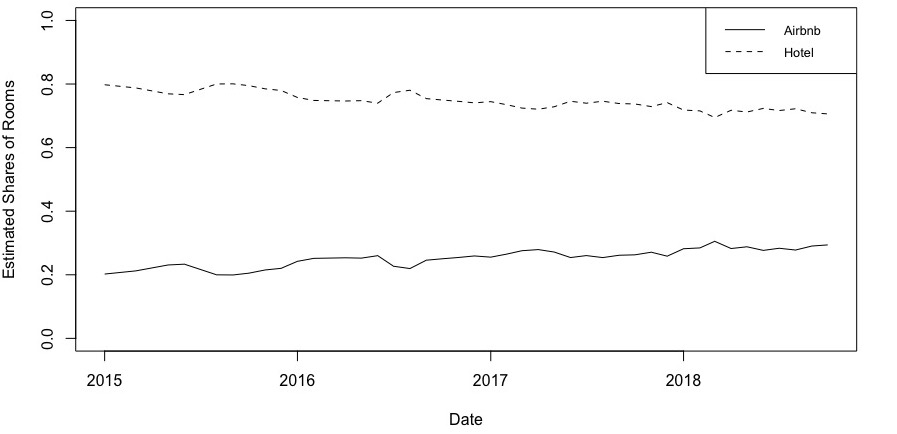
\includegraphics[width=0.7\textwidth]{Figure2.jpeg}
			\end{center}
			\vspace{-.2in}
			\emph{Figure \ref{fig:AirbnbvsHotelGrowth} plots compares the growth of Airbnb and hotel in New York City between 2015 and 2018.}
		\end{figure}

			\par
			A few descriptive statistics are important to understand the accommodation market in New York. Figure \ref{fig:AirbnbvsHotelGrowth} shows Airbnb growth as measured by market shares for the period. In February 2018, Airbnb has over 30\% in estimated room share out of all short-term accommodations (only hotel and Airbnb included). The upward trend shows that Airbnb is taking an increasingly large share out of the NYC accommodation market. This is perhaps not a surprise, as \citet{farronato2018welfare} found New York City to have the highest growth rate among major US cities. Figure \ref{fig:AirbnbvsHotelGrowth} compares the growth trend of hotel vs. Airbnb. The gradually closing gap in room shares between these two accommodation types indicates Airbnb's strong growth. Similarly, Figure \ref{fig:AirbnbSpread} compares Airbnb spread at the start and end of the 4-year period between 2015-2018 in the data. Airbnb listings are geographically dispersing over time, an agreement with results found in \citet{coles2017airbnb}. While most rooms remain concentrated in Manhattan and Brooklyn, Airbnb are geographically dispersing over time, with Queens emerged as a rapidly expanding market. Both statistical and geographical evidence point to the strong growth of the home sharing platform, even 6 years after its entrance\footnote{From Google News searches, the earliest mention of Airbnb in New York City happened in around January 2009}.

		\begin{table}[!htbp]  %Table 1
			\vspace{.2in}
			\begin{center}
  				\caption{Descriptive Statistics for Airbnb Listing Attributes}
				\label{tab:AirbnbStat}
				\scalebox{0.92}{
				\begin{tabular}{@{\extracolsep{5pt}}lccccccc} 
					\\[-1.8ex]\hline 
					\hline \\[-1.8ex] 
					Attribute & \multicolumn{1}{c}{Mean} & \multicolumn{1}{c}{St. Dev.} & \multicolumn{1}					{c}{Min} & \multicolumn{1}{c}{Pctl(25)} & \multicolumn{1}{c}{Median} & \multicolumn{1}{c}{Pctl(75)} & 							\multicolumn{1}{c}{Max} \\ 
					\hline \\[-1.8ex] 
					Price & 150.1 & 209 & 1 & 70 & 110 & 175 & 18,949 \\ 
					Minimum nights & 4.5 & 346 & 1 & 1 & 2 & 3 & 444,443 \\ 
					Reviews per month & 1.4 & 1.5 & 0 & 0.3 & 0.83 & 2.0 & 199 \\ 
					Host listings count & 2.1 & 5.5 & 1 & 1 & 1 & 2 & 174 \\ 
					Number of reviews & 16.4 & 31.1 & 0 & 1 & 4 & 17 & 571 \\ 
					Availability 365 & 151.5 & 144.0 & 0 & 0 & 103 & 310 & 365 \\ 
					Distance from central & 6.4 & 4.0 & 0.03 & 3.2 & 6.0 & 8.5 & 35 \\ 
					\hline \\[-1.8ex] 
					\end{tabular} 
				}
			\end{center}
			\emph{Total observations is about 1.7 million. About 570 observations where price are equal to \$0 were removed. Reviews per month are recorded as monthly averages, while distance from central is point-to-point distance from Empire State Building (in kilometers).}
			\vspace{.1in}
		\end{table}		
			
			\par
			Table \ref{tab:AirbnbStat} shows listing-level descriptive statistics of Airbnb listings. In New York City, an average room costs \$110 per night. This is almost half of average hotel price at \$256 per night. The standard deviation for hotel price is high, demonstrating the range of quality differentiation offered on the home sharing platform. A typical host only has a single room listed, although some have more than one (about 14\% of unique hosts on December 6, 2019). On average, rooms are also available for over 100 days of the next year, more likely to have a long-term impact on the rental market. Table \ref{tab:AirbnbRoomType} and Table \ref{tab:AirbnbBorough} show summary statistics based on room type and borough. Between 2015 and 2018, entire home and apartments make up 51.4\% of all listings while privates room hold about 45\%. Manhattan has the majority of listings at 50.5\%, Brooklyn at 36.4\%, and Queens at 9.5\%. This is accurate with high concentration of Airbnb rooms around Manhattan and Northern Brooklyn in Figure \ref{fig:AirbnbSpread}.
			
		
		\subsection{Hotel and Rental}
			Data of hotel revenue and hotel pricing is obtained from STR Global, a hotel data provider that tracks almost 7 million hotel rooms globally. The raw data contains monthly observations for 771 unique hotels in New York City. STR obtains its data by running a periodic survey of hotels, who voluntarily and confidentially give up their information. Available hotel outcome measures include Occupancy Rate, Average Daily Rate (ADR), and Revenue per Available Room (RevPAR), where RevPAR is  the industry standard used to measure profitability. Additionally, STR also provides hotel equilibrium Supply (number of rooms available) and Demand (number of rooms sold) at an aggregated monthly level.
			
		\begin{table}[!htbp]  %Table 5
			\begin{center}
  				\caption{Descriptive Statistics for Hotel (2015 - 2018)}
				\label{tab:HotelStat} 
				\scalebox{0.88}{ %Wrap inside scale box
				\begin{tabular}{@{\extracolsep{5pt}}lccccccc} 
					\\[-1.8ex]\hline 
					\hline \\[-1.8ex] 
					Statistic & \multicolumn{1}{c}{Mean} & \multicolumn{1}{c}{St. Dev.} & \multicolumn{1}{c}					{Median}&\multicolumn{1}{c}{Min} & \multicolumn{1}{c}{Pctl(25)} & \multicolumn{1}{c}{Pctl(75)} & \multicolumn{1}{c}					{Max} \\ 
					\hline \\[-1.8ex] 
					Occupancy (\%) & 86 & 6.1 & 88.7 & 68.6 & 85.0 & 90.0 & 92 \\ 
					ADR (\$) & 256 & 43.0 & 258.3 & 183.3& 229.4 & 288.3 & 335 \\ 
					RevPAR (\$) & 222 & 48.1 & 227.5 & 129.4 & 204.3 & 258.4 & 302 \\ 
					Supply & 3,462,208 & 192,745 & 3,480,523 & 2,931,124 & 3,344,523 & 3,604,808 & 3,775,056 \\ 
					Demand & 2,984,874 & 309,194 & 3,045,697 & 2,205,451 & 2,896,966 & 3,212,001 & 3,460,560 \\ 
					\hline \\[-1.8ex] 
				\end{tabular} 
				} %Wrap inside scale box 
			\end{center}
			\emph{There are 46 monthly observations between 2015(1) - 2018(10).}
			\vspace{.1in}
		\end{table}
		
			\par
			Table \ref{tab:HotelStat} shows monthly-level descriptive statistics regarding hotels and their outcomes. The 25-percentile and 75-percentile for occupancy rate are 85.0\% and 90.0\%, signaling that New York City hotels are generally booked year-round. Minimum occupancy (68.6\%) took place in January 2015, while maximum occupancy (92\%) took place in October 2018. The standard deviation for monthly hotel rooms available is small at about 192,745 rooms, just under 5\% of total supply. This confirms the static nature of hotel supply.   
			
			\par
			Rental data is provided by StreetEasy and Zillow Research, two searchable online databases for residential property listings and recorded sales (StreetEasy specifically serves New York City). A “rental” is defined as an apartment, house, or any temporary accommodations made available in exchange for money. On StreetEasy, rental terms often last for at least one month, longer-term than the typical Airbnb listing. From January 2000-October 2018, data are made available for New York City includes Sales Inventory, Median Asking Price, and Rent Index, a monthly indicator of rental price growth based on homes in a given neighborhood. Notably, a big portion of rental postings in New York City are unfairly considered as it does not distinguish between regulated and non-regulated apartments. In NYC, over 1 million apartments hold either “rent-controlled” or “rent-stabilized” statuses \footnote{After the NYC housing crisis in 1920, New York State legislature passed a rent-control program designed to keep costs down and limit “baseless” evictions. Rent-controlled apartments current number around 27,000 units and serve a large elderly, low-income population. Whereas rent-controlled apartments impose a rent ceiling, rent-stabilized apartments limit how much a landlord can increase rent each year and give tenants guaranteed rights to renew leases. Source: (https://streeteasy.com/guides/renters-guide/what-is-the-difference-between-rent-controlled-and-rent-stabilized-apartments/.} that make them ineligible for Airbnb.
			
		\begin{table}[!htbp] 
			\begin{center} %Table 7
  				\caption{Rental by Borough}
  				\label{tab:RentalBorough} 
				\begin{tabular}{@{\extracolsep{5pt}} cccccc} 
					\\[-1.8ex]\hline 
					\hline \\[-1.8ex] 
					Borough & \% of Rentals & Mean Inventory & Mean Price & SD Price \\ 
					\hline \\[-1.8ex] 
					Manhattan & $0.54$ & $21,542$ & $3,296$ & $57$ \\
					Brooklyn & $0.33$ & $13,115$ & $2,558$ & $66$ \\ 
					Queens & $0.11$ & $4,539$ & $2,222$ & $54$ \\ 
					Bronx & $0.02$ & $799$ & $1,708$ & $123$ \\ 
					Staten Island & $0.002$ & $83$ & $1,886$ & $138$ \\ 
					\hline \\[-1.8ex] 
				\end{tabular}
			\end{center}
			\emph{Rental inventory and price are broken down at a borough level.}
			\vspace{.1in}
		\end{table}			
			\par
			Table \ref{tab:RentalBorough} provides descriptive statistics for NYC rental market at a borough level. Similar to Airbnb location spread, over half of rental units are located in Manhattan (51\%), following by Brooklyn (36\%), Queens (9.5\%), Bronx (1.7\%), and Staten Island (0.6\%). Clear borough-specific tier in both rent price and quantity is a unique feature to the New York City accommodation market, which Figure \ref{fig:RentalBorough} illustrates. Manhattan, followed by Brooklyn, Queens, Bronx, and Staten Island, in the same order, have the most highest asking rents with the most number of rental units. Figure \ref{fig:AirbnbvsMedianRent} compares the price movements between Airbnb and rental, which shows no seasonal pattern compared to that of hotel.
			
		\subsection{Other Sources}
			Airport passenger data was collected by the Bureau of Transportation Statistics. At a monthly level, the data gives us the total number of passengers arriving at John F. Kennedy International Airport and LaGuardia Airport in Brooklyn. This variable provides is a proxy to account for accommodation demand in New York City. The last source of data, monthly Consumer Price Index in NYC, is extracted from the Bureau of Labor Statistics. This information is used to compute CPI-adjusted price per night for hotel.
			
	\section{Methodology} %Methodology
		I quantify the short-run impact of Airbnb on hotel \& rental as well as the long-term welfare effects under the assumption that Airbnb fully absorbs the deadweight loss created by welfare. I begin by calculating price indexes for the platform using a hedonic regression technique.
		
		\subsection{Airbnb Hedonic Price Index}
			In the data, many attributes influence the price of an Airbnb accommodation: room type, borough, number of reviews, days available in the next year, and number of listings a host owns. Two of these variables were broken down into bins: number of reviews (no reviews, 1-5 reviews, 5-20 reviews, 20-100 reviews, $\geq$100 reviews) and days available ($\leq$100 days, 100-200 days, 200-365 days). Following \citet{coles2017airbnb}, I use the provided geographic coordinates to calculate a variable measuring listing centrality \footnote{Centrality is defined as the distance, in kilometers, away from the Empire State Building. \citet{coles2017airbnb} found it to be a significant determinant of Airbnb price in NYC}. A hedonic regression of Airbnb listings prices allows us to account for heterogeneity in listings types without specifically modeling detailed room type characteristics for New York City \citep{farronato2018welfare}. Taking January 2015 as the base month-year, the hedonic regression is as followed:
			\begin{equation}
				\label{eq:Hedonic}
				\log(p_{it}) = \alpha + \beta_1 m_{it} + \beta_2 n_{it} + \sum_{j=1}^{l}\gamma_j X_{ijt} + \sum_{t=2}^{T}\delta_t D_{it} + \varepsilon_{it}; \ \ i=1,...,N; \ \ t =1,..,42}
			\end{equation}
			
			\par
			where $\log(p_{it}$) is the price of Airbnb listing $i$ during month-year $t$ (42 total month-years between January 2015-December 2018), $m_{it}$ is the number of properties owned by host of listing $i$ (continuous attribute), $n_{it}$ is the distance from the Empire State Building (continuous attribute), $X_{ijt}$ is attribute $j$ of listing $i$ at time $t$ (categorical attributes), and $D_{it}$ are the month-year time dummy variables where $D_{it}$  = 1 if the listing $i$ was posted during month-year $t$ ($D_{it}$ = 0 is January 2015). $\gamma_j$ and $\delta_j$ provide multiple regression coefficients, where $\delta_j$ are estimations of Airbnb price indexes and our coefficients of interest \citep{kunovac2008use}.
			
			\par
			Under this model, the changes in Airbnb listing price over time are fully reflected by coefficients $\delta_j$ of the month-year dummy variables. Since they are not affected by the fact that an Airbnb accommodation might be of different room types, reputation, or borough, they can be treated the as the pure prices of Airbnb over the period. Price index for month-year $t$ can be calculated as $\hat{Index}_t$ = 100*$e^{\delta_j}$, with $Index_0$ = 100 for the base month-year. 
			
			\par
			Figure \ref{fig:AirbnbPrice} draws plot of NYC Airbnb price index over time. After a price dip at the start of 2016, Airbnb price has been gradually increasing, topping at a 6\% increase by the end of 2018. While subjected to some seasonality, Figure \ref{fig:AirbnbvsHotelPrice} shows that Airbnb has much less price variability compared to hotel. The seasonal variability shows that hotel managers are price-setting experts, adapting to short-term demand to maximize profits while maintaining healthy occupancy rates.
			
		\begin{figure}[!htbp] %Figure 4
			\begin{center}
				\caption{NYC Airbnb Price Movement 2015-2018}
				\label{fig:AirbnbPrice}
				\includegraphics[width=0.7\textwidth]{Figure4.jpeg}
			\end{center}
			\vspace{-.2in}
			\emph{Figure \ref{fig:AirbnbPrice} plots the price movement of Airbnb in New York City based on the hedonic $\delta$ coefficients in Equation \ref{eq:Hedonic}.}
		\end{figure}
			
			\begin{figure}[!htbp] %Figure 5
			\begin{center}
				\caption{NYC Airbnb vs. Hotel Price Movement 2015-2018}
				\label{fig:AirbnbvsHotelPrice}
				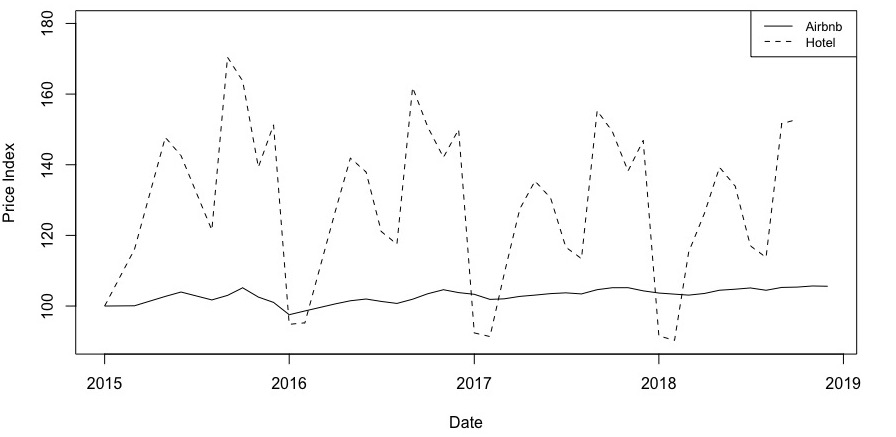
\includegraphics[width=0.7\textwidth]{Figure5.jpeg}
			\end{center}
			\vspace{-.2in}
			\emph{Hotel price indexes are the month-year changes of average daily rate over time multiplied by 100 (index of base month-year, January 2015, is 100). We assume that hotel attributes do not significantly change form period-to-period.}
		\end{figure}

		\subsection{The Short-Run: Effects of Peer Entry on Hotel Outcomes} %Short-run Hotel
			In this section, we estimate the effects of Airbnb supply on different outcome measures of hotels using an OLS linear regression. Here, the number of arriving passengers at local airports act as the proxy for short-term accommodation demand. This model follows closely a similar estimation by \citet{farronato2018welfare}. The baseline regression model is:
			\begin{equation}
				\label{eq:HotelSR}
				y_t = \alpha + \beta_1 \log(Q_{{Airbnb}_t}) + \beta_2 \log(P_{{Airbnb}_t}) + \delta \log(AirportPassenger_t) + \gamma X_t + \varepsilon_t
			\end{equation}
			
			\par
			where $y_t$ is one of three hotel outcomes $\in$\{log(OccupancyRate), log(ADR), log(RevPAR)\} at month $t$, $\log(Q_{{Airbnb}_t})$ is Airbnb listing quantity, $\log(P_{{Airbnb}_t})$ is Airbnb hedonic price index, \$\log(AirportPassengers_t)$ is the number of total arriving passengers at JFK and LaGuardia airports, and $X_t$ captures the monthly fixed effects. $X_t$ is necessary since demand for accommodation and travel is often associated with seasonality.
			
			\par
			Here, the coefficients of interest, $\beta_1$, has the following interpretation: a percentage change in Airbnb supply affects hotel outcome by $\beta$*100 percent change. This is essentially the average short-run elasticity of hotel outcomes to Airbnb supply in the sample \citep{farronato2018welfare}. By including $\log(P_{Airbnb})$ as another explanatory variable, I am interested to see if price changes in short-term home sharing might influence hotel outcomes. Table \ref{tab:RegHotelOutcomes} shows the results of the baseline regression model, which will be discussed in Section 6.2.
			  
		\subsection{The Long-Run: Market Equilibrium and Welfare Calculation} %Long-run Hotel
			As discussed in Section 3.1, our model assumes that the deadweight loss (DWL) incurred by a hotel price increase is fully absorbed by home sharing. The quantification strategy is an estimation of DWL savings made by Airbnb during the period. Data availability for hotel equilibrium demand, estimated and provided by STR Global, makes this calculation possible.
			
			\subsubsection{Hotel Equilibrium Demand}
				At equilibrium, hotel demand is the total number of hotel rooms sold by hotel respondents in the survey conducted monthly by STR.
			
			\subsubsection{Effects of Airbnb Entry on Hotel Price}
				In this section, I want to measure the price change ($\bigtriangleup P$) of hotel before and after Airbnb enters New York City. Here, hotel price is adjusted for inflation by the following formula: $(\frac{AverageDailyRate}{CPI_i}*{CPI_{Jan 2000}}})$, where $CPI_i$ is the Consumer Price Index for NYC during month-year $i$. January 1, 2009 is set as the benchmark for Airbnb's entrance in the city. A regression of the entrance time dummy variable with month fixed effects on inflation-adjusted ADR gives us the average price change ($\bigtriangleup P$) before and after Airbnb entrance. On average, I estimate hotel per night to be \$10.9 lower after Airbnb entry. Results of this regression are in Table \ref{tab:HotelBefore}.
		
			\subsubsection{Price Elasticities}
				Price elasticities calculation for hotel supply is as followed:
				\begin{equation}
					\begin{split}
				 		\bigtriangleup Q_{Hotel} & = \bigtriangleup  P_{{Hotel}_t} + \bigtriangleup P_{{Airbnb}_t} + MonthFE_t + \epsilon_t\\
						log(DemandHotel_t) & = log(PriceHotel_t) + log(PriceAirbnb_t) + MonthFE_t + \epsilon_t
					\end{split}
				\end{equation}
			
				\par
				where $\log(DemandHotel_t)$ is the number of hotel rooms sold in time $t$, $\log(PriceHotel_t)$ is hotel price at equilibrium, $\log(PriceAirbnb_t)$ is the estimated Airbnb price index, and $MonthFE_t$ is the month fixed effects to account for seasonal accommodation demand. Results for the above equation, including a few elasticity alterations with $\log(PriceRent_t)$ and $\log(QuantityAirbnb_t)$, are outlined in Table \ref{tab:HotelPriceElasticity}. From the first column, my model estimates $\varepsilon_{Hotel}$ to be equal -0.15\% and $\varepsilon_{Airbnb}$ to be equal 2.69\%.
			
			\subsubsection{Deadweight Loss}
				We follow the equation presented in Section 3 to quantify welfare:
				\begin{equation}
					\begin{split}
					Welfare & = DWL = \frac{1}{2} \times  \bigtriangleup Q \times \bigtriangleup P \\
					& = \frac{1}{2} \times \frac{Q}{P} \times {\bigtriangleup P}^2 \times \varepsilon_{Hotel}
				\end{split}
			\end{equation}
				
				\par
				Table \ref{tab:Welfare} lists estimations of Airbnb daily DWL savings at a month-year level. For New York City in October 2018 (Q = 115,352, P = 205), for instance, Airbnb provides an extra \$7,845 in daily welfare and \$235,350 in aggregated monthly welfare.
		
		\subsection{Effects of Peer Entry on Rental Outcomes} %Impact of Rental
			For rental, I use the same predictor variable, Airbnb supply, to determine its relationship with different rental incomes. I include location fixed effects for both borough and neighborhood in NYC.
			
			\subsubsection{Effects by Borough}
				Baseline OLS model by borough:
				\begin{equation}
					\label {eq:RentalBorough}
					y_{it} = \alpha + \beta \log(QuantityAirbnb_{it}) + \delta B_{it} + \gamma X_t + \varepsilon_{it}
				\end{equation}
			
				\par
				where $y_{it}$ is one of two rental outcomes $\in$\{log(RentalInventory), log(MedianAskingPrice)\} in borough $i$ at month $t$, $\log(QuantityAirbnb_{it})$ is the number of Airbnb listings available, $B_{it}$ captures the borough fixed effects, and $X_t$ captures the monthly fixed effects. $B_{it}$ controls for borough while $X_t$ is necessary since accommodation demand changes seasonally.
	
				\par
				The coefficient of interest, $\beta$, has the following interpretation: a percentage change in Airbnb supply affects rental outcome by $\beta$*100 percent change. Table \ref{tab:RegRentalBorough} shows the results of our model.
			
			\subsubsection{Effects by Neighborhood}
				Baseline OLS model by neighborhood:
				\begin{equation}
					\label {eq:RentalNeighbour}
					y_{it} = \alpha + \beta \log(QuantityAirbnb_{it}) + \delta N_{it} +\gamma X_t + \varepsilon_{it}
				\end{equation}
			
				\par
				where $y_{it}$ is one of 6 rental outcomes $\in$\{log(RentalInventory), log(AllAskingRent),\\ log(OneBedroomRent), log(TwoBedroomRent), log(ThreeBedroomRent), log(StudioRent)} in neighborhood $i$ at month $t$, $\log(QuantityAirbnb_{it})$ is the number of Airbnb listings available, $N_{it}$ captures the neighborhood fixed effects, and $X_t$ captures the month fixed effects. Same as above, $X_t$ is necessary since accommodation demand changes seasonally.
				
				\par
				The coefficient of interest, $\beta$, has the following interpretation: a percentage change in Airbnb supply affects rental outcome by $\beta$*100 percent change. At the neighborhood level, data availability allows us to look at the impact across rental types. Table \ref{tab:RegRentalNeighbor} shows the results of the model.
		
			 
	\section{Results} %Results
		\subsection{Airbnb Price Determinants}
		
		\begin{table}[!htbp] 
			\begin{center} %Table 8
  				\caption{Hedonic Regression of Airbnb Listing Attributes on Price}
  				\label{tab:Hedonic} 
				\begin{tabular}{@{\extracolsep{5pt}}lc} 
					\\[-1.8ex]\hline 
					\hline \\[-1.8ex] 
 					& \multicolumn{1}{c}{\textit{Dependent variable:}} \\ 
					\cline{2-2} 
					\\[-1.8ex] & $\log(Price)$ \\ 
					\hline \\[-1.8ex]
  					Room type: Private room & $-$0.752$^{***}$ (0.001) \\ 
  					Room type: Shared room & $-$1.075$^{***}$ (0.002) \\ 
  					Review bin: No reviews & 0.146$^{***}$ (0.001) \\ 
  					Review bin: 1-5 reviews & 0.0005 (0.001) \\ 
  					Review bin: 20-100 reviews & $-$0.016$^{***}$ (0.001) \\ 
  					Review bin: $\geq$100 reviews & $-$0.077$^{***}$ (0.002) \\ 
  					Availability bin: $\leq$100 days & $-$0.117$^{***}$ (0.001) \\ 
  					Availability bin: 200-365 days & 0.084$^{***}$ (0.001) \\ 
  					Borough: Manhattan & 0.154$^{***}$ (0.003) \\ 
  					Borough: Brooklyn & $-$0.008$^{***}$ (0.003) \\ 
  					Borough: Queens & $-$0.074$^{***}$ (0.003) \\ 
  					Borough: Staten Island & 0.213$^{***}$ (0.005) \\ 
  					Host Listings Count & $-$0.003$^{***}$ (0.0001) \\ 
  					Distance from Empire State & $-$0.040$^{***}$ (0.0001) \\ 
  					Constant & 5.281$^{***}$ (0.004) \\ 
 					\hline \\[-1.8ex] 
					Month-year FE (n=43; base year=January 2015)\\
					Observations & 1,778,041 \\ 
					R$^{2}$ & 0.531 \\ 
					Adjusted R$^{2}$ & 0.531 \\ 
					Residual Std. Error & 0.458 (df = 1777983) \\ 
					\hline 
					\hline \\[-1.8ex] 
					\textit{Note:}  & \multicolumn{1}{r}{$^{*}$p$<$0.1; $^{**}$p$<$0.05; $^{***}$p$<$0.01} \\ 
				\end{tabular} 
			\end{center}
		\end{table}
		
		 	The hedonic regression model explains 53.1\% of variability in the data. Room type, reputation (reviews), location (borough), and centrality (distance from Empire State Building) are all important determinants of Airbnb price in New York City, showing statistical and economic significance. Airbnb rooms that are private and shared, for example, are about 75\% and 108\% cheaper than rooms that are an entire home or apartment. For every kilometer located farther away from central Manhattan, a listing becomes 4.0\% cheaper. With Bronx as the base, listings in Manhattan is 15.4\% more expensive while listings in Queens is 7.4\% cheaper. Listing with no reviews are about 0.13\% more expensive, and listings available for less than 100 days are about 11.7\% lower in price. For review and availability, we should expect the possibility of two-way causation: that price of an Airbnb listing can affect both its booking frequency and number of guest reviews. With the inclusion of distance from Empire State variable, which should be highly correlated with Manhattan borough, the coefficient on Manhattan dummy variable remains highly and statistically significance.
			
		\subsection{Home Sharing \& Hotel}
			Results from Equation 3 is presented in Table \ref{tab:RegHotelOutcomes}. OLS regression model finds a 10\% increase in Airbnb supply to be associated with a 1.3\% decrease in hotel price and a 1.2\% decrease in hotel revenue. As home sharing asserts a competitive pressure on hotel, the consumers are expected to benefit, especially during periods of high travel demand. Additionally, the fact that Airbnb supply has no bearing on hotel occupancy signals that the two goods have little substitution relationship. There are two potential reasons for this phenomenon. (1) Since Airbnb's NYC entrance in 2009, hotel managers have come up with strategies to cope with Airbnb growth. (2) New York City hotel targets consumers at a higher willingness-to-pay level, so the two goods are differentiated in the highly populated city.
			
			\par
			Across the board, Airbnb price is found to have a strong positive association with hotel outcomes. An increase in Airbnb price is estimated to raise occupancy, price per night, and revenue by 0.6\%, 0.6\%, and 1.3\%, increasing hotel demand, price, and profitability. Basic economic principles for substitute goods dictate a reasonable outcome: that an increase in price for one good leads to an increase in demand for the substitute. However, due to the insignificant relationship between home sharing supply and hotel occupancy, another likely explanation is that the positive association between Airbnb price and hotel outcomes are biased towards peak periods for travel demand, where ($Q_{Hotel}$, $P_{Hotel}$, $Q_{Airbnb}$, $P_{Airbnb}$) are expected to surge. In New York City, a popular destination worldwide, local airport passenger fails to be an adequate control variable that encompasses all demand for accommodation\footnote{In \citet{farronato2018welfare}, for example, a control for one-week lag of Google searches for hotels was found to be helpful in capturing accommodation demand.}.
			
		\begin{table}[!htbp]  %Table 9
			\begin{center}
  				\caption{Impact of Airbnb Supply on Hotel Outcomes}
				\label{tab:RegHotelOutcomes}
				\begin{tabular}{@{\extracolsep{5pt}}lccc} 
					\\[-1.8ex]\hline 
					\hline \\[-1.8ex] 
 					& \multicolumn{3}{c}{\textit{Dependent variable:}} \\ 
					\cline{2-4} 
					\\[-1.8ex] & $\log(Occupancy)$ & $\log(ADR)$ & $\log(RevPAR)$ \\ 
					\\[-1.8ex] & (1) & (2) & (3)\\ 
					\hline \\[-1.8ex] 
 					$\log(QuantityAirbnb)$ & 0.010 (0.022) & $-$0.127$^{***}$ (0.038) & $-$0.117$^{**}$ (0.048) \\ 
  					$\log(PriceAirbnb) & 0.646$^{***}$ (0.171) & 0.631$^{**}$ (0.301) & 1.276$^{***}$ (0.378) \\ 
  					$\log(TotalNYC)$ & 0.140 (0.125) & 0.446$^{*}$ (0.220) & 0.583$^{**}$ (0.276) \\ 
 					Constant & $-$0.907 (1.834) & $-$3.001 (3.230) & $-$8.474$^{**}$ (4.053) \\ 
 					\hline \\[-1.8ex] 
					Month FE & Yes & Yes & Yes\\
					Observations & 39 & 39 & 39 \\ 
					R$^{2}$ & 0.985 & 0.991 & 0.993 \\ 
					Adjusted R$^{2}$ & 0.976 & 0.986 & 0.988 \\ 
					Residual Std. Error (df = 24) & 0.012 & 0.021 & 0.027 \\ 
					\hline 
					\hline \\[-1.8ex] 
					\textit{Note:}  & \multicolumn{3}{r}{$^{*}$p$<$0.1; $^{**}$p$<$0.05; $^{***}$p$<$0.01} \\ 
				\end{tabular} 
			\end{center}
			\emph{Table \ref{tab:RegHotelOutcomes} shows linear regression results for the impact of Airbnb quantity on different hotel outcomes provided in Equation \ref{eq:HotelSR}.}
		\end{table}
		
			
			\par
			From Table \ref{tab:HotelPriceElasticity}, the signs on different price elasticity coefficients are all in the expected directions. Excluding rental price, an increase in hotel price is associated with a 0.02\$ decrease in hotel demand; an increase in Airbnb price is associated with a 1.1\% increase in hotel demand. In the long run, welfare created by home sharing is small from a deadweight loss perspective. As shown in Table \ref{tab:Welfare}, daily savings average just about \$8,000 during 2015-2018, a tiny fraction of hotel revenue. Given our method and limits related to data collection, including the lack of granularity and unobserved equilibrium supply for Airbnb, we should cautiously infer this result.
			
		\subsection{Home Sharing \& Rental}
			Results from Equation 6 and Equation 7 are presented in Table \ref{tab:RegRentalBorough} and Table \ref{tab:RegRentalNeighbor}. At a borough level, a 10\% increase in Airbnb supply is associated with a 2.42\% increase in rental inventory and a 0.86\% increase in median asking price. The same effects are found at a neighborhood level, where home sharing is found to raise rents across all types of rental units considered, including one-bedroom, two-bedroom, three-bedroom, and studio (Table \ref{tab:RegRentalNeighbor}). While this finding agrees with previous literature, the consistently positive association between Airbnb and rental inventory comes as a surprise (against the hypothesis proposed in Section 3.2). Here, data limitation is once again a potential cause. On a particular day, through online platforms such as StreetEasy and Airbnb, a host can simultaneously list her home for short- and long-term rental before choosing the option that maximizes her utility. Taking all listed rooms as home sharing supply means an inclusion of properties that, in reality, are unavailable. It is likely that my model is grossly overestimating Airbnb supply at equilibrium. Additionally, while $R^2$ are beyond 96\% in both the borough-controlled and neighborhood-controlled models, omitted variable bias remains a concern. Data on new constructions in a specific borough or neighborhood over time could make for a helpful control variable.
			
		\begin{table}[!htbp]   %Table 13
			\vspace{.2in}
			\begin{center}
  			\caption{Impact of Airbnb Supply on Rental Outcomes by Borough} 
			\label{tab:RegRentalBorough}
			\begin{tabular}{@{\extracolsep{5pt}}lcc} 
				\\[-1.8ex]\hline 
				\hline \\[-1.8ex] 
				& \multicolumn{2}{c}{\textit{Dependent variable:}} \\ 
				\cline{2-3} 
				\\[-1.8ex] & $\log(RentalInventory)$ & $\log(AskingRent)$ \\ 
				\\[-1.8ex] & (1) & (2)\\ 
				\hline \\[-1.8ex] 
 				$\log(QuantityAirbnb)$ & 0.242$^{***}$ (0.042) & 0.086$^{***}$ (0.010) \\ 
 				Constant & 5.053$^{***}$ (0.268) & 6.873$^{***}$ (0.066) \\ 
				\hline \\[-1.8ex]
				Borough FE (n=5) & Yes & Yes\\
				Month FE & Yes & Yes \\
				Observations & 210 & 210 \\ 
				R$^{2}$ & 0.994 & 0.972 \\ 
				Adjusted R$^{2}$ & 0.993 & 0.970 \\ 
				Residual Std. Error (df = 193) & 0.169 & 0.041 \\ 
				\hline 
				\hline \\[-1.8ex] 
				\textit{Note:}  & \multicolumn{2}{r}{$^{*}$p$<$0.1; $^{**}$p$<$0.05; $^{***}$p$<$0.01} \\ 
			\end{tabular} 
			\end{center}
			\emph{Table \ref{tab:RegRentalBorough} shows linear regression results for Equation \ref{eq:RentalBorough}, which includes both borough and month fixed effects.}
		\end{table} 
		
			
	\section{Robustness}
		\subsection*{Modeling Airbnb Price with Random Effects}
		In Equation \ref{eq:Hedonic}, month-year fixed effects were applied to the hedonic regression to account for time-invariant characteristics of Airbnb, assuming that each listing is an independent observation. In the data, however, many listings are repeated as they were available at different points in time. It is reasonable to expect correlation among the listings with the same unique ID. To ensure that listing-specific heteroskedasticity does not have any major bearing predicting Airbnb price, I account for between-listing error through a regression with random effects:

		\begin{equation}
			\label{eq:HedonicRE}
			\log(p_{it}) = \alpha + \beta_1 m_{it} + \beta_2 n_{it} + \sum_{j=1}^{l}\gamma_j X_{ijt} + \sum_{t=2}^{T}\delta_t D_{it} + \mu_{it} + \varepsilon_{it}
		\end{equation}
		
		\par
		where $\log(p_{it}$) is the price of $i$ Airbnb listing in month-year $t$, $m_{it}$ is the number of properties owned by host of listing $i$, $n_{it}$ is the distance from the Empire State Building, $X_{ijt}$ is attribute $j$ of listing $i$ at time $t$, $D_{it}$ are the month-year time dummy variables ($\gamma_j$ and $\delta_j$ both provide multiple regression coefficients), and $\mu_{it}$ is the between-listing error term for listing $i$ at time $t$.

		\par
		From the original hedonic regression, the random effects model has significantly more explanatory power, explaining over 71\% in the data. It provides coefficients of comparable magnitude in case all cases except for room type. The difference is noticeable, as renting private and shared rooms is only about 33\% and 46\% cheaper than renting an entire home or apartment (compared to 75\% and 108\% before). Additionally, the signs on different review bins have been changed to the opposite direction. A listing that has 1-5 reviews is found to be 0.7\% less expensive than a listing with 5-20 reviews. Though listing-specific heteroskedasticity does seem to have some impact on room type and peer reviews, the comparable magnitude of most dependent variables suggests that the model in Equation \ref{eq:Hedonic} is adequate in estimating Airbnb price. From Figure \ref{fig:AirbnbPriceRE}, price indexes produced by the two models follow each other closely, with price separation remains within 5\%. In the original model, the positive slope for price indexes post-2016 are perhaps biased towards Airbnb listings that were persistently high-priced, thus remaining unbooked over time. The inclusion of random fixed effects teases out members of this group, slightly flattening out price indexes post-2016.
		 
		\begin{table}[!htbp] 
			\begin{center} %Table 10
  				\caption{Hedonic Regression with Random Effects}
  				\label{tab:HedonicRE} 
				\begin{tabular}{@{\extracolsep{5pt}}lc} 
					\\[-1.8ex]\hline 
					\hline \\[-1.8ex] 
					& \multicolumn{1}{c}{\textit{Dependent variable:}} \\ 
					\cline{2-2} 
					\\[-1.8ex] & $\log(Price)$ \\ 
					\hline \\[-1.8ex]
  					Room type: Private room & $-$0.331$^{***}$ (0.001) \\ 
  					Room type: Shared room & $-$0.455$^{***}$ (0.002) \\ 
  					Review bin: No reviews & 0.007$^{***}$ (0.001) \\ 
  					Review bin: 1-5 reviews & $-$0.007$^{***}$ (0.0004) \\ 
  					Review bin: 20-100 reviews & 0.006$^{***}$ (0.0005) \\ 
  					Review bin: $\geq$ 100 reviews & 0.011$^{***}$ (0.001) \\
  					Availability bin: $\leq$ 100 days & $-$0.009$^{***}$ (0.0005) \\ 
  					Availability bin: 200-365 days & 0.017$^{***}$ (0.0005) \\ 
   					Borough: Manhattan & 0.180$^{***}$ (0.009) \\ 
  					Borough: Brooklyn & $-$0.044$^{***}$ (0.008) \\ 
 					Borough: Queens & $-$0.087$^{***}$ (0.009) \\ 
  					Borough: Staten Island & 0.285$^{***}$ (0.017) \\ 
 					Host Listings Count & $-$0.001$^{***}$ (0.0001) \\ 
   					Distance from Empire State & $-$0.044$^{***}$ (0.0003) \\ 
  					Constant & 5.109$^{***}$ (0.009) \\ 
 					\hline \\[-1.8ex]
					Month-year (n=43; base year=January 2015)\\
					Random Effects & Yes \\
					Observations & 1,773,385 \\ 
					R$^{2}$ & 0.716 \\ 
					Adjusted R$^{2}$ & 0.716 \\ 
					\hline 
					\hline \\[-1.8ex] 
					\textit{Note:}  & \multicolumn{1}{r}{$^{*}$p$<$0.1; $^{**}$p$<$0.05; $^{***}$p$<$0.01} \\ 
				\end{tabular} 
			\end{center}
			\emph{Table \ref{tab:HedonicRE} shows regression results for the random-effects model of Airbnb price in Equation \ref{eq:HedonicRE}.}
		\end{table}

		
	\section{Conclusion}
		As sharing economy platforms continue to grow in size, so does the magnitude of its impact on markets and consumers. My work focuses on Airbnb and its economics in New York City, an understudied urban market. While pursuing a deadweight loss strategy to quantify welfare, I provide insights that partially agree with previous findings. For instance, in the context of the incumbent industry, namely hotel, I find little evidence for hotel and Airbnb being substitute goods. As experts, NYC hotel managers seem to have skillfully adapted to market conditions, keeping occupancy high year-round while coping with the competitive pressure asserted by home sharing. With home sharing taking up an increasingly notable room shares, hotels are forced to reduce price, thus becoming less profitable as a result. This phenomenon benefits the consumers, especially those that cannot afford hotel in the hypothetical absence of home sharing. Positive, though small, welfare effects are quantified in the form of hotel deadweight loss during the 2015-2018 period. In the context of rental, the existence of Airbnb allows hosts to choose the term structure that provides utility. In the short term, though home sharing does not deplete rental housing supply, it is found to raise rents across all types of units considered, making rental less affordable. Lastly, a hedonic regression technique shows low price variability for Airbnb and uncovers important price determinants of a NYC accommodation. Under two different models, room type, reputation, availability, borough, and centrality remain helpful in predicting Airbnb price.
		
		\par
		My work has some limitations that confine its scope. First, one must recognize that findings found in the paper are only representative of New York City during the selected time period. We cannot generalize conclusions found here to directly apply them to other urban areas where economic, political, and cultural characteristics are distinctive. All additional studies quantifying region-specific impact of home sharing could be useful and should be welcome. Second, in many cases, the lack of data granularity limits the confidence level of my model results. Instead of monthly, a daily-level dataset would significantly improve this study. Finally, web-scraped data does not provide information on whether a listing is booked. As economists have few tools to determine actual Airbnb supply at equilibrium, it is challenging to accurately measure the welfare effects of home sharing. Based on previous literature, gaining access to proprietary data seems to be the best solution for these last two points.
		
		\par
		While the paper quantifies welfare effects from a deadweight loss perspective, welfare could also be examined through other lenses, including the quantification of host surplus and guest surplus, or the negative externalities incurred on the local community such as noise, congestion, and competition for parking \citep{farronato2018welfare, gurran2017tourists}. As Uber, Lyft, and Airbnb continue to grow, more effort should be made to understand the modern-life impact of these sharing economy platforms.
		
		\par
		Similar to other works, results found in my paper have implications for policy makers. Regardless of sector, region- and market-specific characteristics suggest that policies around the sharing economy should only be considered at a municipal level. The impact of home sharing on hotel in New York City, where substitution is low, shall be different from its impact in Texas. To the extent that taxation of these platforms proves to be challenging, local governments might lose out on revenue in the short run (though it is possible for platforms to bring in increased demand to local businesses in a city \citep{zervas2017rise}). Our point remains that the net economic impact of the new market phenomenon is hard to quantify. Applying a federal, one-size-fits-all policy to restrict these platforms should perhaps be discouraged as it can be harmful towards consumer and societal welfare.
		

	\clearpage %END OF WRITING
	
	\linespread{1} %Back to single space
	
	\section*{Tables} %Tables
	\addcontentsline{toc}{section}{Tables}%Add to table of content


		\begin{table}[!htbp] 
			\begin{center} %Table 2
  				\caption{Airbnb Listings by Room Type} 
  				\label{tab:AirbnbRoomType} 
				\begin{tabular}{@{\extracolsep{5pt}} cccccc} 
					\\[-1.8ex]\hline 
					\hline \\[-1.8ex] 
					Room Type & N & \% of Listings* & Median Price & Mean Price\\ 
					\hline \\[-1.8ex] 
					Entire home/apt & $160,215$ & $0.51$ & $170$ & $210$ \\ 
					Private room & $140,289$ & $0.45$ & $75$ & $89$ \\ 
					Shared room & $11,235$ & $0.04$ & $49$ & $65$ \\ 
					\hline \\[-1.8ex] 
				\end{tabular} 
				\vspace{.1in}
				
				\caption{Airbnb Listings by Borough}  %Table 3
				\label{tab:AirbnbBorough} 
				\begin{tabular}{@{\extracolsep{5pt}} ccccc} 
					\\[-1.8ex]\hline 
					\hline \\[-1.8ex] 
					Borough & N & \% of Listings* & Median Price & Mean Price\\ 
					\hline \\[-1.8ex] 
					Manhattan & $157,569$ & $0.51$ & $149$ & $186$ \\
					Brooklyn & $113,488$ & $0.36$ & $90$ & $118$ \\
					Queens & $29,686$ & $0.095$ & $75$ & $97$ \\
					Bronx & $5,178$ & $0.017$ & $60$ & $81$ \\ 
					Staten Island & $1,771$ & $0.006$ & $69$ & $121$ \\ 
					\hline \\[-1.8ex] 
				\end{tabular} 
			\end{center}
			\emph{In Table \ref{tab:AirbnbRoomType} and Table \ref{tab:AirbnbBorough}, listings are unique by ID and price. If a listing was listed at 2 different prices, both are considered in the summary tables.}
		\end{table}
		
		\begin{table}[!htbp] %Table 4
			\begin{center}
				\caption{Airbnb Listings by Availability Bin} 
				\label{tab:AirbnbAvailability}
				\begin{tabular}{@{\extracolsep{5pt}} ccccc} 
					\\[-1.8ex]\hline 
					\hline \\[-1.8ex] 
					Availability Bin & N & \% of Listings* & Median Price & Mean Price \\ 
					\hline \\[-1.8ex] 
					$\leq100$ days & $143,854$ & $0.461$ & $110$ & $140$ \\ 
					100 - 200 days & $69,406$ & $0.223$ & $120$ & $151$ \\ 
					200 - 365 days & $163,584$ & $0.525$ & $115$ & $159$ \\ 
					\hline \\[-1.8ex] 
				\end{tabular} 
			\end{center}
			\emph{In Table \ref{tab:AirbnbAvailability}, listings are unique by ID, availability bin, and price. We consider repeated IDs that might have different availability and prices. In our data, number of unique listings by ID is only 162,584 units.}
		\end{table}	
		

		\begin{table}[!htbp]  %Table 10
			\begin{center}
  				\caption{Hotel Price Before Airbnb Entry (Jan 2000-Oct 2018)}
				\label{tab:HotelBefore}
				\begin{tabular}{@{\extracolsep{5pt}}lc} 
					\\[-1.8ex]\hline 
					\hline \\[-1.8ex] 
 					& \multicolumn{1}{c}{\textit{Dependent variable:}} \\ 
					\cline{2-2} 
					\\[-1.8ex] & $ADR_{adjusted}$\\ 
					\hline \\[-1.8ex] 
 					BeforeAirbnb & 10.910$^{***}$ (2.636) \\ 
  					Constant & 144.688$^{***}$ (4.747) \\ 
 					\hline \\[-1.8ex]
					Month FE & Yes\\
					Observations & 226 \\ 
					R$^{2}$ & 0.602 \\ 
					Adjusted R$^{2}$ & 0.580 \\ 
					Residual Std. Error & 19.788 (df = 213) \\ 
					\hline 
					\hline \\[-1.8ex] 
					\textit{Note:}  & \multicolumn{1}{r}{$^{*}$p$<$0.1; $^{**}$p$<$0.05; $^{***}$p$<$0.01} \\ 
				\end{tabular} 
			\end{center}
			\emph{Dependent variable is hotel CPI-adjusted average daily price.}
		\end{table}
					
		\begin{table}[!htbp]  %Table 11
			\begin{center}
  				\caption{Hotel Price Elasticities}
				\label{tab:HotelPriceElasticity}
				\begin{tabular}{@{\extracolsep{5pt}}lccc} 
					\\[-1.8ex]\hline 
					\hline \\[-1.8ex] 
 					& \multicolumn{3}{c}{\textit{Dependent variable:}} \\ 
					\cline{2-4} 
					\\[-1.8ex] & \multicolumn{3}{c}{$\log(HotelDemand)$} \\ 
					\\[-1.8ex] & (1) & (2) & (3)\\ 
					\hline \\[-1.8ex] 
 					$\log(PriceHotel)$ & $-$0.153$^{**}$ (0.063) & $-$0.020 (0.026) & $-$0.013 (0.028) \\ 
  					$\log(PriceAirbnb)$ & 2.690$^{***}$ (0.415) & 1.092$^{***}$ (0.202) & 1.143$^{***}$ (0.212) \\ 
  					$\log(PriceRent)$ &  &  & 0.100 (0.119) \\ 
  					$\log(QuantityAirbnb)$ &  & 0.225$^{***}$ (0.018) & 0.216$^{***}$ (0.021) \\ 
  					Constant & 3.001 (2.012) & 7.401$^{***}$ (0.842) & 6.766$^{***}$ (1.135) \\ 
 					\hline \\[-1.8ex] 
 					Month FE & Yes & Yes & Yes\\
					Observations & 42 & 42 & 42 \\ 
					R$^{2}$ & 0.913 & 0.988 & 0.988 \\ 
					Adjusted R$^{2}$ & 0.872 & 0.981 & 0.981 \\ 
					Residual Std. Error & 0.037 (df = 28) & 0.014 (df = 27) & 0.014 (df = 26) \\ 
					\hline 
					\hline \\[-1.8ex] 
					\textit{Note:}  & \multicolumn{3}{r}{$^{*}$p$<$0.1; $^{**}$p$<$0.05; $^{***}$p$<$0.01} \\ 
				\end{tabular} 
			\end{center}
			\emph{Hotel demand is the number of hotel rooms sold at equilibrium. Airbnb price indexes are the $\delta$ coefficients in our hedonic regression, while hotel price indexes are the price movements of hotel average daily rate.}
		\end{table}		 
		
		\begin{table}[!htbp] %Table 12
			\begin{center}
  			\caption{Hotel Deadweight Loss Savings} 
  			\label{tab:Welfare}
			\scalebox{0.93}{ %begin of scales box
			%\begin{spacing}{1.25}
			\begin{tabular}{@{\extracolsep{5pt}} ccccc} 
				\\[-1.8ex]\hline 
				\hline \\[-1.8ex]  
				Time & Rooms Sold/Day & ADR Adjusted (\$) & DWL Adjusted (\$) & DWL (\$) \\ 
				\hline \\[-1.8ex] 
				Jan 2015 & $74,157$ & $134$ & $5,022$ & $7,237$ \\ 
				Mar 2015 & $90,156$ & $156$ & $5,261$ & $7,619$ \\ 
				May 2015 & $98,713$ & $199$ & $4,525$ & $6,588$ \\ 
				Jun 2015 & $96,941$ & $192$ & $4,604$ & $6,715$ \\ 
				Aug 2015 & $98,232$ & $163$ & $5,476$ & $7,982$ \\ 
				Sep 2015 & $97,469$ & $229$ & $3,873$ & $5,657$ \\
				Oct 2015 & $100,729$ & $220$ & $4,168$ & $6,079$ \\ 
				Nov 2015 & $91,359$ & $187$ & $4,442$ & $6,466$ \\ 
				Dec 2015 & $96,525$ & $203$ & $4,321$ & $6,264$ \\ 
				Jan 2016 & $79,162$ & $127$ & $5,654$ & $8,210$ \\ 
				Feb 2016 & $77,552$ & $128$ & $5,514$ & $8,023$ \\ 
				Apr 2016 & $96,687$ & $170$ & $5,166$ & $7,567$ \\ 
				May 2016 & $102,182$ & $191$ & $4,877$ & $7,162$ \\ 
				Jun 2016 & $100,450$ & $185$ & $4,932$ & $7,258$ \\ 
				Jul 2016 & $103,602$ & $163$ & $5,794$ & $8,521$ \\ 
				Aug 2016 & $103,315$ & $158$ & $5,954$ & $8,772$ \\ 
				Sep 2016 & $102,660$ & $218$ & $4,295$ & $6,338$ \\ 
				Oct 2016 & $104,724$ & $202$ & $4,707$ & $6,950$ \\ 
				Nov 2016 & $100,862$ & $191$ & $4,808$ & $7,111$ \\ 
				Dec 2016 & $104,151$ & $202$ & $4,702$ & $6,961$ \\ 
				Jan 2017 & $85,743$ & $124$ & $6,285$ & $9,356$ \\ 
				Feb 2017 & $82,775$ & $123$ & $6,136$ & $9,160$ \\ 
				Mar 2017 & $100,864$ & $146$ & $6,267$ & $9,352$ \\ 
				Apr 2017 & $102,758$ & $171$ & $5,459$ & $8,158$ \\ 
				May 2017 & $106,485$ & $182$ & $5,326$ & $7,967$ \\ 
				Jun 2017 & $105,363$ & $175$ & $5,466$ & $8,190$ \\ 
				Jul 2017 & $108,978$ & $157$ & $6,327$ & $9,460$ \\ 
				Aug 2017 & $107,679$ & $152$ & $6,430$ & $9,634$ \\ 
				Sep 2017 & $107,261$ & $209$ & $4,677$ & $7,045$ \\
				Oct 2017 & $110,850$ & $201$ & $5,024$ & $7,554$ \\ 
				Nov 2017 & $104,408$ & $186$ & $5,116$ & $7,687$ \\ 
				Dec 2017 & $109,049$ & $197$ & $5,028$ & $7,560$ \\ 
				Jan 2018 & $92,834$ & $123$ & $6,868$ & $10,372$ \\ 
				Feb 2018 & $87,932$ & $121$ & $6,595$ & $10,013$ \\ 
				Mar 2018 & $108,419$ & $155$ & $6,369$ & $9,669$ \\ 
				Apr 2018 & $105,542$ & $170$ & $5,664$ & $8,622$ \\ 
				May 2018 & $112,616$ & $187$ & $5,476$ & $8,368$ \\ 
				Jun 2018 & $109,352$ & $180$ & $5,530$ & $8,455$ \\ 
				Jul 2018 & $111,317$ & $157$ & $6,442$ & $9,846$ \\ 
				Aug 2018 & $112,275$ & $153$ & $6,683$ & $10,229$ \\ 
				Sep 2018 & $108,112$ & $204$ & $4,828$ & $7,417$ \\
				Oct 2018 & $115,352$ & $205$ & $5,113$ & $7,845$ \\ 
				\hline \\[-1.8ex] 
			\end{tabular} 
			} %end of scale box
			%\end{spacing}
			\end{center}
			\emph{Each deadweight loss saving value is a daily estimation of Airbnb welfare for New York City during that month-year.}
		\end{table}

		
		\begin{sidewaystable}[!htbp]  %Table 14
			\begin{center}
  			\caption{Impact of Airbnb Supply on Rental Outcomes by Neighborhood}
			\label{tab:RegRentalNeighbor}
			\scalebox{0.81}{
			\begin{tabular}{@{\extracolsep{5pt}}lcccccc} 
				\\[-1.8ex]\hline 
				\hline \\[-1.8ex] 
 				& \multicolumn{6}{c}{\textit{Dependent variable:}} \\ 
				\cline{2-7} 
				\\[-1.8ex] & $\log(RentalInventory)$ & $\log(AskingRent)$ & $\log(OneBedRent)$ & $\log(TwoBedRent)$ & 				$\log(ThreeBedRent)$ & $\log(StudioRent)$ \\ 
				\\[-1.8ex] & (1) & (2) & (3) & (4) & (5) & (6)\\ 
				\hline \\[-1.8ex] 
				$\log(QuantityAirbnb)$ & 0.204$^{***}$ (0.012) & 0.067$^{***}$ (0.003) & 0.064$^{***}$ (0.003) & 0.048$^{***}$ (0.003) & 0.040$^{***}$ (0.004) & 0.028$^{***}$ (0.007) \\ 
  				Constant & 5.91$^{***}$ (0.103) & 7.25$^{***}$ (0.019) & 7.15$^{***}$ (0.019) & 7.45$^{***}$ (0.019) & 7.72$^{***}$  (0.027) & 7.42$^{***}$ (0.044) \\ 
				 \hline \\[-1.8ex]
				Neighborhood FE & Yes & Yes & Yes & Yes & Yes & Yes \\
				Month FE & Yes & Yes & Yes & Yes & Yes & Yes \\
				Observations & 5,546 & 4,204 & 1,312 & 1,296 & 1,190 & 987 \\ 
				R$^{2}$ & 0.960 & 0.959 & 0.989 & 0.989 & 0.986 & 0.964 \\ 
				Adjusted R$^{2}$ & 0.959 & 0.957 & 0.988 & 0.989 & 0.986 & 0.962 \\ 
				Residual Std. Error & 0.408 (df = 5389) & 0.064 (df = 4066) & 0.034 (df = 1268) & 0.035 (df = 1252) & 0.042 (df = 					1146) & 0.048 (df = 944) \\ 
				\hline 
				\hline \\[-1.8ex] 
				\textit{Note:}  & \multicolumn{6}{r}{$^{*}$p$<$0.1; $^{**}$p$<$0.05; $^{***}$p$<$0.01} \\ 
			\end{tabular}
			}
			\end{center}
			\emph{Table \ref{tab:RegRentalNeighbor} shows linear regression results of different rental outcomes with neighborhood and monthly fixed effects. Dependent variables in column (1) and column (2) are rental inventory and median rent on aggregate. Dependent variables in columns (3), (4), (5), and (6) are rents broken down by one-bedroom, two-bedroom, three-bedroom, and studio rentals.}
		\end{sidewaystable} 	 
	\clearpage %END OF TABLES

	\section*{Figures} %Figures
	\addcontentsline{toc}{section}{Figures}%Add to table of content

	%\setcounter{figure}{0}
		\begin{figure}[!htb] %Figure 1
			\begin{center}
				\caption{NYC Growth of Airbnb (2015-2018)}
				\label{fig:AirbnbGrowth}
				\includegraphics[width=0.7\textwidth]{Figure1.jpeg}
			\end{center}
			\vspace{-.2in}
			\emph{Figure \ref{fig:AirbnbGrowth} plots the growth of Airbnb in New York City between 2015 and 2018. The y-axis is the estimated monthly share of Airbnb supply out of all rooms available (hotel and Airbnb) for short-term accommodations. This closely resembles the estimation calculated by \citet{farronato2018welfare}.} 
		\end{figure}
		
	
		\begin{figure}[!htb]% Figure 3
    			\begin{center}
				\caption{Map of Airbnb Spread in New York City}%
				\label{fig:AirbnbSpread}
    				\subfloat[January 1st, 2015]{{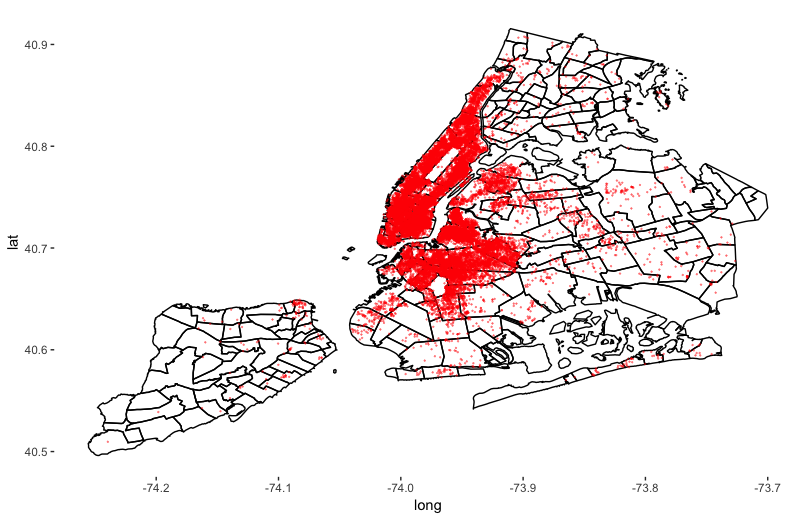
\includegraphics[width=14cm]{Figure3a.png} }}%
    				\qquad
   			 	\subfloat[December 6th, 2018]{{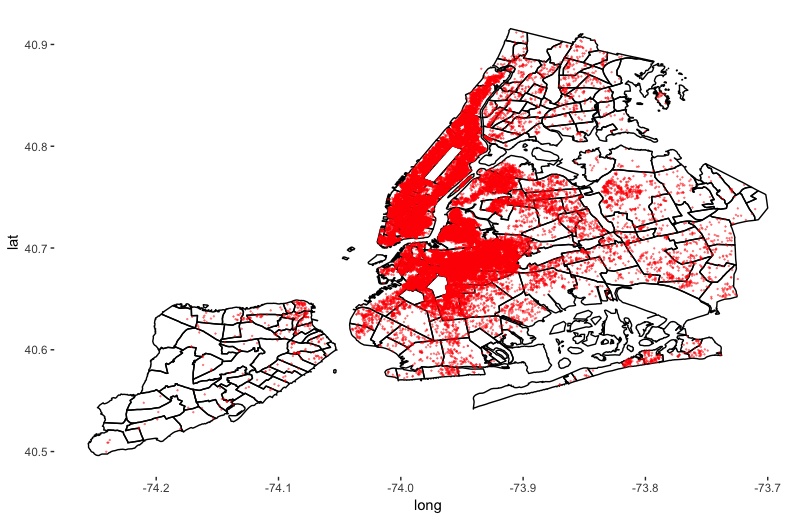
\includegraphics[width=14cm]{Figure3b.png} }}%
   			 \end{center}
			 \emph{The first map draws Airbnb spatial distribution during the earliest scrape in our data on January 1st, 2015. The second map draws the latest scrape on December 6th, 2018. Maps were drawn using library "ggplot2" in R.}
		\end{figure}
		
		
		\begin{figure}[!htb] %Figure 6
			\begin{center}
				\caption{Rental Characteristics by Borough}
				\label{fig:RentalBorough}
				\includegraphics[width=0.7\textwidth]{Figure6.jpeg}
			\end{center}
			\vspace{-.2in}
			\emph{Figure \ref{fig:RentalBorough} uses monthly observations of inventory and rent price by borough.}
		\end{figure}
		
		\begin{figure}[!htb] %Figure 7
			\begin{center}
				\caption{NYC Airbnb vs. Median Rent Movement (2015-2018)}
				\label{fig:AirbnbvsMedianRent}
				\includegraphics[width=0.7\textwidth]{Figure7.jpeg}
			\end{center}
			\vspace{-.2in}
			\emph{Figure \ref{fig:AirbnbvsMedianRent} compares the price movement of Airbnb and rental in New York City.}
		\end{figure}
		
			\begin{figure}[!htb] %Figure 5
			\begin{center}
				\caption{Price Index Comparison for Random Effects Model}
				\label{fig:AirbnbPriceRE}
				\includegraphics[width=0.7\textwidth]{Figure8.jpeg}
			\end{center}
			\vspace{-.2in}
			\emph{FE model is the original hedonic regression in Equation \ref{eq:Hedonic}. RE model is the regression with random effects in Equation \ref{eq:HedonicRE}}.
		\end{figure}

	\clearpage %END OF FIGURES


	%\section*{Appendix}%Appendix
	%\addcontentsline{toc}{section}{Appendix}%Add to table of content


	\clearpage
	
	\addcontentsline{toc}{section}{References}%Add to table of content
	\bibliography{References} %References
	\bibliographystyle{apacite}
	\nocite{*}
	\clearpage

\end{document}





